\documentclass[11pt]{article}
\usepackage{amsmath, amssymb}
\usepackage{geometry}
\geometry{margin=1in}
\usepackage{fancyhdr}
\usepackage{lastpage}
\usepackage{parskip} % Better paragraph spacing
\usepackage{titlesec} % Better section formatting
\usepackage{graphicx}
\usepackage{float}
\usepackage[most]{tcolorbox}
\usepackage{lmodern}
\usepackage{caption}
\usepackage{hyperref}
\usepackage{listings}
\usepackage{xcolor}
\usepackage{tikz}
\usetikzlibrary{automata, positioning, arrows.meta}

\definecolor{codegreen}{rgb}{0,0.6,0}
\definecolor{codegray}{rgb}{0.5,0.5,0.5}
\definecolor{codepurple}{rgb}{0.58,0,0.82}
\definecolor{backcolour}{rgb}{0.95,0.95,0.92}

% Define code styling
\lstdefinestyle{mystyle}{
    backgroundcolor=\color{backcolour},
    commentstyle=\color{codegreen},
    keywordstyle=\color{magenta},
    numberstyle=\tiny\color{codegray},
    stringstyle=\color{codepurple},
    basicstyle=\ttfamily\footnotesize,
    breakatwhitespace=false,
    breaklines=true,
    captionpos=b,
    keepspaces=true,
    numbers=left,
    numbersep=5pt,
    showspaces=false,
    showstringspaces=false,
    showtabs=false,
    tabsize=2
}

\lstset{style=mystyle}

% Define commands for reusable content
\newcommand{\coursename}{CS-550 Formal Verification}
\newcommand{\lecturenum}{02}
\newcommand{\lecturedate}{\today}
\newcommand{\professor}{Viktor Kuncak}

\hypersetup{colorlinks=true,linkcolor=blue,urlcolor=blue}

% Configure section spacing
\titlespacing*{\section}{0pt}{2ex plus 1ex minus .2ex}{1.5ex plus .2ex}
\titlespacing*{\subsection}{0pt}{1.5ex plus 1ex minus .2ex}{1ex plus .2ex}
% Header / Footer
\pagestyle{fancy}
\fancyhf{}
\fancyhead[L]{\coursename}
\fancyhead[R]{Lecture \lecturenum}
\fancyfoot[L]{EPFL - Computer Science}
\fancyfoot[C]{Author: Jonathan Dutoit}
\fancyfoot[R]{Page \thepage\ of \pageref{LastPage}}

\begin{document}

\begin{center}
  {\large EPFL - Computer Science} \\[0.5em]
  {\Large \textbf{\coursename}} \\[0.5em]
  {\large Lecture \lecturenum\ --- \lecturedate} \\[0.5em]
  {\large Author: Jonathan Dutoit} \\[0.5em]
  {\large Professor: \professor} \\[0.5em]
\end{center}

\vspace{1.5cm}

\begin{center}
  {\LARGE \textbf{Finite Systems Expressed with Formulas}}
\end{center}
\vspace{0.5cm}

\textbf{Symbolic model checking}: Explicitly storing all reachable states is often too expensive. Instead, represent state sets compactly using formulas or data structures. Two important techniques for finite-state systems are \textbf{bounded model checking}, which uses \textbf{SAT solvers} to . search for errors within a fixed bound, and \textbf{BDD}-based reachability checking, which computes reachable-state sets symbolically until a fixed point is reached. 

\section*{Boolean Functions: Encoding FTS (Finite Transition Systems)}

Consider a deterministic finite-state transition system: \textit{M = (S, I, r, A)}. 
If we pick $n \geq log_2|S|$ and $m \geq log_2|A|$, we can represent the finite-state transition system using boolean functions: 
\begin{itemize}
	\item Each element of \textit{S} as $\bar{s} \in \{0, 1\}^{n}$, so $S = \{0, 1\}^{n}
	\item Each element of \textit{A} as $\bar{a} \in \{0, 1\}^{n}$, so $A = \{0, 1\}^{n}
	\item Initial states $I \subseteq S$ by the characteristic function $\{0, 1\}^{n} \rightarrow \{0, 1\}$
	\item Deterministic transition relation $r \subseteq S \times X \times S$ as a function $(S \times A) \rightarrow S$, that is, $\{0, 1\}^{n} \times \{0, 1\}^{m} \to \{0, 1\}^{n}$
\end{itemize}

\begin{figure}[H]
\centering
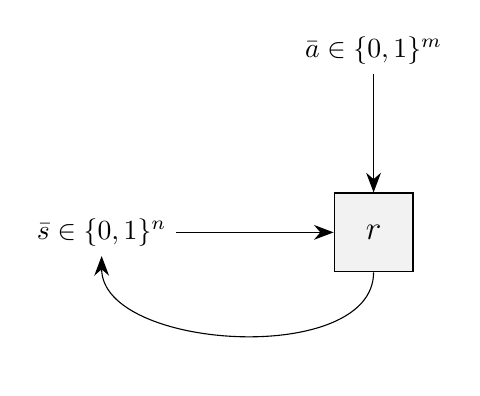
\begin{tikzpicture}[
    node distance=2.2cm, auto,
    >={Stealth[length=2.5mm]},
    block/.style={rectangle, draw, fill=gray!10, minimum width=1cm, minimum height=1cm, font=\large},
    term/.style={font=\normalsize}
]

  % Central block
  \node[block] (r) {$r$};

  % Top input ($\bar{a} \in \{0,1\}^m$)
  \node[term, above=1.5cm of r] (a) {$\bar{a} \in \{0,1\}^m$};
  \path[->] (a) edge (r);

  % Left input ($\bar{s} \in \{0,1\}^n$)
  \node[term, left=2cm of r] (s) {$\bar{s} \in \{0,1\}^n$};
  \path[->] (s) edge (r);

  % Bottom feedback loop curving back to the left input/state
  \draw[->] (r.south) .. controls +(0,-1.2) and +(0,-1.2) .. (s.south);

\end{tikzpicture}
\end{figure}
(For non-deterministic systems, we represent \textit{r} as $(S \times A \times S \to \{0, 1\}$)

\textbf{Example: Blinking Lights:} 

$S = \{0, 1\}$ (1 = "light on") $\quad$ $A = \{0, 1\}$ (1 = "toggle light") $\quad$ $I(s) = (s = 0)$ $\quad$ $r(s, a) = s \oplus a$ 

\begin{figure}[H]
\centering
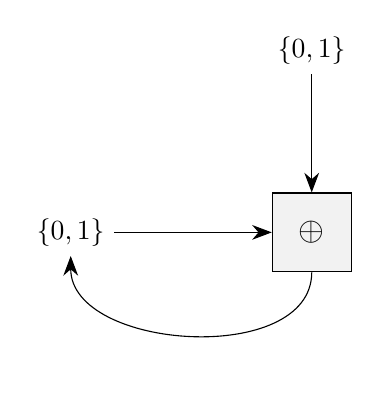
\begin{tikzpicture}[
    node distance=2.2cm, auto,
    >={Stealth[length=2.5mm]},
    block/.style={rectangle, draw, fill=gray!10, minimum width=1cm, minimum height=1cm, font=\large},
    term/.style={font=\normalsize}
]
  \node[block] (xor) {$\oplus$};

  \node[term, above=1.5cm of xor] (a) {$\{0, 1\}$};
  \path[->] (a) edge (xor);

  \node[term, left=2cm of xor] (l) {$\{0, 1\}$};
  \path[->] (l) edge (xor);

  \draw[->] (xor.south) .. controls +(0,-1.2) and +(0,-1.2) .. (l.south);

\end{tikzpicture}
\end{figure}

% Quick centered image
\begin{figure}[H]
    \centering
    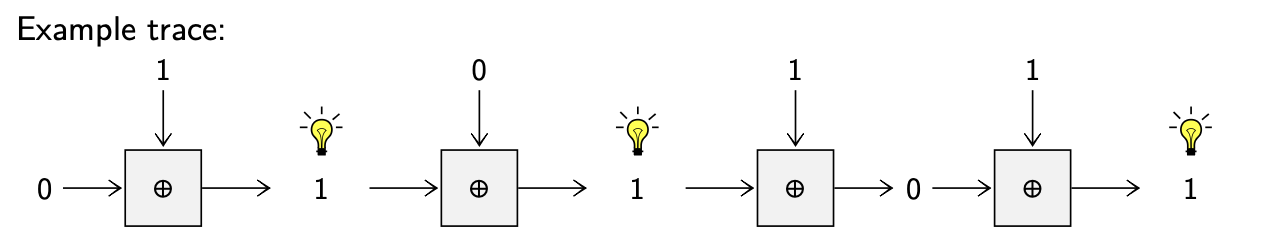
\includegraphics[width=0.8\textwidth]{images/blinking-lights}
    \label{fig:LABEL}
\end{figure}


\subsection*{Boolean Function Representation: Table}

Let \textit{r}: $\{0, 1\}^{n} \times \{0, 1\}^{m} \to \{0, 1\}^{n}$. The table list each of the $\{0,1\}^{n+m}$ inputs and specify the result. When $s, a \in \{0, 1\}^{4}$ and represent addition of 4-bit non-negative integers modulo 16:

\[
\left.
\begin{array}{c|c|c}
s & a & r(s,a) \\
\hline
0000 & 0000 & 0000 \\
0000 & 0001 & 0001 \\
0000 & 0010 & 0010 \\
\multicolumn{3}{c}{\dots} \\
0001 & 0000 & 0001 \\
0001 & 0001 & 0010 \\
\multicolumn{3}{c}{\dots} \\
1111 & 1111 & 1110
\end{array}
\right\}
2^{4+4} = 256 \text{ columns}
\]

In general, we cannot do better than truth table (there are that many different functions), but truth table always has bad representation size, even for functions like $+_4$. 

\textbf{\textcolor{red}{What happens in practice}}: in verification we don't deal with random systems. We care about meaningful systems that have a more concise representation and are computable functions. 

\subsection*{Boolean Function Representation: Formulas}

\begin{tcolorbox}[
    enhanced,
    frame hidden,
    borderline west={2pt}{0pt}{black},
    boxsep=5pt,
    left=8pt
]
Let $r \subseteq \{0, 1\}^{n} \times \{0, 1\}^{m} \times \{0, 1\}^{n}$. \textbf{Definition.} Without loss of generality, we can always represent \textit{r} by a propositional formula in disjunctive normal form: 
\[
	\bigvee_{((v_1, ..., v_n),(u_1,...,u_m), (v_1', ..., v_n'))\in r}\left(\bigwedge_{1 \leq i \leq n}s_i^{v_i} \land \bigwedge_{1 \leq 1 \leq m} a_i^{u_i} \land \bigwedge_{1 \leq 1 \leq n} (s'_i)^{v_i'}\right)
.\] 

Where we represent the condition 
\[
	((s_1, ..., s_n), (a_1, ..., a_m), (s_1', ..., s_n')) \in r
.\] 

by writing a propositional formula with variable $s_1, ..., s_n, \, a_1, ..., a_m, \, s_1', ..., s_n'$ that is \textit{true} precisely when the tuple belongs to \textit{r}, and if \textit{p} is a propositional variable and $v \in \{0, 1\}$ then we define $p^{v}$ by $p^{1} = p$ and $p^{0} = \neg p$
\end{tcolorbox}

\textbf{Example: Blinking Lights}

$S = \{0, 1\}$ (1 = "light on") $\quad$ $A = \{0, 1\}$ (1 = "toggle light") $\quad$ $I(s) = (s = 0)$ $\quad$ $r(s, a) = s \oplus a$

\begin{figure}[H]
\centering
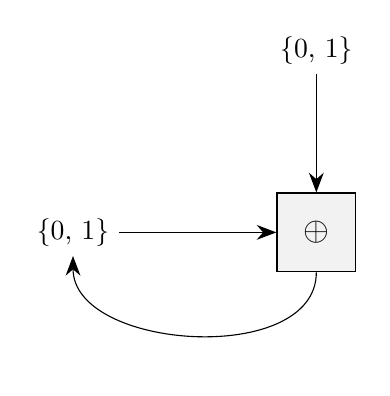
\begin{tikzpicture}[
    node distance=2.2cm, auto,
    >={Stealth[length=2.5mm]},
    block/.style={rectangle, draw, fill=gray!10, minimum width=1cm, minimum height=1cm, font=\large},
    term/.style={font=\normalsize}
]
  \node[block] (xor) {$\oplus$};

  \node[term, above=1.5cm of xor] (a) {\{0, 1\}};
  \path[->] (a) edge (xor);

  \node[term, left=2cm of xor] (l) {\{0, 1\}};
  \path[->] (l) edge (xor);

  \draw[->] (xor.south) .. controls +(0,-1.2) and +(0,-1.2) .. (l.south);
\end{tikzpicture}
\end{figure}


Formula R represents condition $(s, a, s') \in r$: 
\[
	\begin{array}{c|c}
	\textit{r} \quad (relation) & \textit{R} \quad (formula) \\
	\hline
	\{(0, 0, 0), & (\neg s \land \neg a \land \neg s') \, \lor \\
	(0, 1, 1), & (\neg s \land a \land s') \, \lor \\
	(1, 0, 1), & (s \land \neg a \land s') \, \lor \\
	(1, 1, 0)\} & (s \land a \land \neg s') 
\] 

\newpage
\section*{Propositional (Boolean) Logic}

Propositional logic is a language for representing Boolean functions $f : \{0, 1\}^{n} \to \{0, 1\}$. Grammar of formulas: 
\[
P ::= x \, | \, 0 \, | \, 1 \, | \, P \land P \, | \, \neg P \, | \, P \lor P \, | \, P \oplus P \, | \, P \to P \, | P \leftrightarrow P  
.\] 

where x denotes variables (identifiers). Corresponding Scala trees: 

\begin{lstlisting}[language=Octave]
sealed abstract class Expr
case class Var(id: Identifier) extends Expr
case class BooleanLiteral(b: Boolean) extends Expr
case class And(e1: Expr, e2: Expr) extends Expr
case class Or(e1: Expr, e2: Expr) extends Expr
case class Not(e: Expr) extends Expr
\end{lstlisting}


\begin{tcolorbox}[
    enhanced,
    frame hidden,
    borderline west={2pt}{0pt}{black},
    boxsep=5pt,
    left=8pt
]
\textbf{Definition.} An environment \textit{e} is a partial map from propositional variables to $\{0, 1\}$. For a vector of \textit{n} boolean variables $\bar{p} = (p_1, ..., p_n)$ and $\bar{v} = (v_1, ..., v_n) \in \{0, 1\}^{n}$, we denote $[\bar{p} \mapsto \bar{v}]$ the environment \textit{e} given by $e(pi) = v_i$ for $i \leq i \leq n$. \\

We write $e \models F$, and define $[\![ F ]\!]_e = 1$, to denote that \textit{F} is true in environment \textit{e}, otherwise we define $[\![F]\!]_e = 0$. 
\end{tcolorbox}

\textbf{Example: } Let $e = \{\(a, 1), (b, 1), (c, 0)\}$ and \textit{F} be $a \land (\neg b \lor c)$. Then: 
\[
	[\![a \land (\neg b \lor c)]\!]_e = e(a) \land (\neg e(b) \lor e(c)) = 1 \land (\neg 1 \lor 0) = 0
.\] 

The general definition is recursive for assigning truth values to formulas:
\[
\begin{align*}
	&\ [\![x]\!]_e = e(x) \\
	&\ [\![0]\!]_e = 0 \\
	&\ [\![1]\!]_e = 1 \\
	&\ [\![F_1 \land F_2]\!]_e = [\![F_1]\!]_e \land [\![F_2]\!]_e \\
	&\ [\![\neg F_1]\!]_e = \neg [\![F_1]\!]_e
\end{align*}
.\]


\subsection*{Satisfiability Problem}

\begin{tcolorbox}[
    enhanced,
    frame hidden,
    borderline west={2pt}{0pt}{black},
    boxsep=5pt,
    left=8pt
]
\textbf{Definition.} Formula \textit{F} is \textit{satisfiable}, iff there \textbf{exists} \textit{e} such that $[\![F]\!]_e = 1$. \\ 
Otherwise we call \textit{F} \textit{unsatisfiable}: when there does not exist \textit{e} such that $[\![F]\!]_e = 1$, that is, for all \textit{e}, $[\![F]\!]_e = 0$. \\

SAT is a problem: given a propositional formula. determine whether it is satisfiable. The problem is \textbf{decidable} because given \textit{F} we can compute its variables \textit{FV(F)} and it suffices to look at the $2^{n}$ environments for \textit{n = FV(F)}. The problem is NP-complete, but useful heuristics exist. 
\end{tcolorbox}

\textbf{Example:} Let \textit{F} be a $a \land (\neg b \lor c)$. Then \textit{F} is satisfiable, with e.g. $e = \{(a, 1), (b, 0), (c, 0)\}$. Its negation of $\neg F = \neg a \lor (b \land \neg c)$, is also satisfiable, with e.g. $e = \{(a, 0), (b, 0), (c, 0) \}$. 

A SAT solver is a program that, given boolean formula \textit{F}, either: 
\begin{itemize}
	\item returns \textbf{sat}, and, optionally, returns one environment \textit{e} such that $[\![F]\!]_e = 1$, or
	\item returns \textbf{unsat} and, optionally, returns a \textbf{proof} that no satisfying assignment exists. Either the program tries every environment possibility, or uses some observations to evaluate a more concise equivalent formula. 
\end{itemize}

\subsection*{Syntax vs Semantics}
\begin{itemize}
    \item \textbf{Syntax (Form \& Structure):} The symbols and mechanical rules for writing formulas.
    \begin{itemize}
        \item $(p \land q)$ is a valid formula; substitution ($F[p := q]$) is pure text replacement.
    \end{itemize}

    \item \textbf{Semantics (Meaning \& Truth):} What those symbols actually evaluate to under an interpretation.
    \begin{itemize}
        \item Assigning $p = \text{True}$ and $q = \text{False}$, or checking if an environment $e$ satisfies a formula ($e \models F$).
    \end{itemize}
\end{itemize}

\subsection*{Substitutions}

Let \textit{F, G} be propositional formulas and \textit{c} a propositional variable. \\ 
Let $F[c := G]$ denote the result of replacing in \textit{F} each occurrence of \textit{c} by \textit{G} recursively. 

\textbf{Example $F[c := \neg p]$}
\begin{figure}[htbp]
    \centering
    % --- Original Tree F ---
    \begin{minipage}{0.45\textwidth}
        \centering
        \textbf{Original Formula $F = (c \land q) \lor c$} \\[1em]
        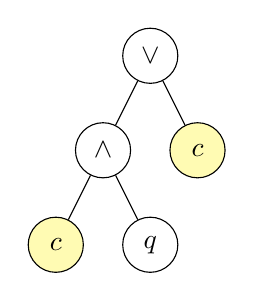
\begin{tikzpicture}[scale=0.8, every node/.style={circle, draw, minimum size=7mm, inner sep=2pt}]
            \node {$\lor$}
                child { node {$\land$}
                    child { node[fill=yellow!30] {$c$} }
                    child { node {$q$} }
                }
                child { node[fill=yellow!30] {$c$} };
        \end{tikzpicture}
    \end{minipage}
    \hfill
    % --- Result Tree F[c := G] ---
    \begin{minipage}{0.45\textwidth}
        \centering
        \textbf{After Substitution $F[c := \neg p]$} \\[1em]
        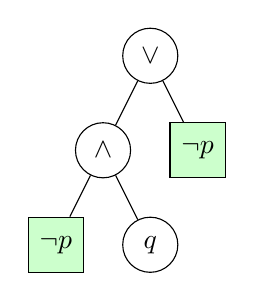
\begin{tikzpicture}[scale=0.8, every node/.style={circle, draw, minimum size=7mm, inner sep=2pt}]
            \node {$\lor$}
                child { node {$\land$}
                    child { node[rectangle, draw, fill=green!20] {$\neg p$} }
                    child { node {$q$} }
                }
                child { node[rectangle, draw, fill=green!20] {$\neg p$} };
        \end{tikzpicture}
    \end{minipage}
\end{figure}

The general definition is: 
\[
\begin{align*}
	c[c := G] &\ = G \\ 
	(F_1 \land F_2)[c := G] &\ =  F_1[c := G] \land F_2[c := G] \\
	(F_1 \lor F_2)[c := G] &\ = F_1[c := G] \lor F_2[c := G] \\
	(\neg F_1)[c := G] &\ = \neg (F_1[c := G]) 
\end{align*}
.\] 

We also generalize to simultaneous replacement of many variables, $F[\bar{c} := \bar{G}].$ \\ 
Then following formulas are equivalent (have same truth for all free variables): 
\begin{itemize}
	\item $F[c := G]$
	\item $\exists c.((c = G) \land F)$ \emph{satisfied only if F evaluates to true when c is replaced inside G} 
	\begin{itemize}
		\item The existential quantifier $(\exists c)$ looks across all possible values for c. 
		\item The subformula requires \textbf{both} \textit{c = G} and \textit{F} to be true
		\item Because of \textit{c = G}, the only value of \textit{c} that can possibly satisfy this condition is whatever \textit{G} evaluates to
		\item When \textit{c} takes that specific value, checking if \textit{F} is true is the exact same thing as taking \textit{F} and replacing every \textit{c} with \textit{G}.
	\end{itemize}
	\item $\forall c. ((c = G) \to F)$ \emph{The only value of c that actually tests F is when C = G. This forces F to hold precisely where c has been replaced by G}
	\begin{itemize}
		\item If c \textbf{is not} equal to \textit{G}, then the premise (\textit{c = G}) is \textbf{false}. In logic, a false premise makes an implication \textbf{automatically} (vacuously) true. So all other values of \textit{c} get a free pass.
		\item The only time the premise is actually tested is when \textit{c} \textbf{does} equal G.
		\item When \textit{c = G}, the implication forces F to be true. 
	\end{itemize}
\end{itemize}

Note: free variables are the variables occurring in the formula minus quantified ones (c). 

\subsection*{Free Variables for Quantified Boolean Formulas}

Quantified boolean formulas (QBF) are build from propositional variables and constants 0, 1 using $\land, \lor, \neg, \to, \leftrightarrow, \exists, \forall$ (We also write $=$ for $\leftrightarrow$). \\
A boolean formula is a QBF without quantifiers $\forall, \exists$. \\
Definition of free variables of a formula: 
\[
	\begin{align*}
		FV(v) &\ = \{v\} \text{ when v is a propositional variable} \\ 
		FV(F_1 \land F_2) &\ =  FV(F_1) \cup FV(F_2) \\ 
		FV(F_1 \lor F_2) &\ = FV(F_1) \cup FV(F_2) \\ 
		FV(F_1 \to F_2) &\ = FV(F_1) \cup FV(F_2) \\ 
		FV(\neg F_1) &\ = FV(F_1) \\ 
		FV(\exists v. F_1) &\ = FV(F_1) \setminus \{v\} \\
		FV(\forall v. F_1) &\ = FV(F_1) \setminus \{v\}
	\end{align*}
.\] 

\subsection*{Validity and Equivalence}

\begin{tcolorbox}[
    enhanced,
    frame hidden,
    borderline west={2pt}{0pt}{black},
    boxsep=5pt,
    left=8pt
]
\textbf{Definition.} Formula \textit{F} is \emph{valid}, iff for all \textit{e}, $e \models F \leftrightarrow [\![F]\!]_e = 1.$  \\ 

\textbf{Observation}: \textit{F} \textbf{is valid iff} $\neg F$ \textbf{is unsatisfiable}. \emph{Unsatisfiable means always evaluates to false. Hence, if not F is always false, then F is always true, a.k.a, valid. }
\end{tcolorbox}

\begin{tcolorbox}[
    enhanced,
    frame hidden,
    borderline west={2pt}{0pt}{black},
    boxsep=5pt,
    left=8pt
]
\textbf{Definition.} Formulas \textit{F} and \textit{G} are equivalent iff for every \textit{e} that defines all variables in $FV(F) \cup FV(G)$, we have: $e \models F$ iff $e \models G$. \\ 

\textbf{Observation:} \textit{F} and \textit{G} are equivalent iff $F \leftrightarrow G$ is valid. \emph{Means that for any arbitrary environment, F and G hold the same truth value}. 
\end{tcolorbox}

$\exists p. F$ us equivalent to $F[p := 0] \lor F[p := 1]$ whereas $\forall p. F$ to $F[p := 0] \land F[p := 1]$.

\newpage
\section*{Boolean Function Representation: Circuits}

Formulas correspond to \textit{trees}: variables are leaves, operations internal nodes. \\
More efficient representation that exploits sharing: directed acyclic graphs (DAGs). We can view DAGs as formulas with \textit{auxiliary} variable definitions. 

\begin{figure}[htbp]
    \centering
    
    % --- 1. Syntax Tree ---
    \begin{minipage}{0.31\textwidth}
        \centering
        \textbf{1. Syntax Tree} \\[0.5em]
        \small $F = (c \land q) \lor (c \land q)$ \\[1em]
        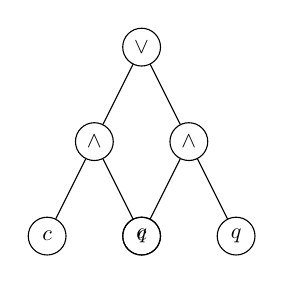
\begin{tikzpicture}[scale=0.8, transform shape, every node/.style={circle, draw, minimum size=6mm, inner sep=1pt}]
            \node (or) {$\lor$}
                child { node {$\land$}
                    child { node {$c$} }
                    child { node {$q$} }
                }
                child { node {$\land$}
                    child { node {$c$} }
                    child { node {$q$} }
                };
        \end{tikzpicture}
    \end{minipage}
    \hfill
    % --- 2. Shared DAG ---
    \begin{minipage}{0.31\textwidth}
        \centering
        \textbf{2. Shared DAG} \\[0.5em]
        \small Exploiting subformula sharing \\[1em]
        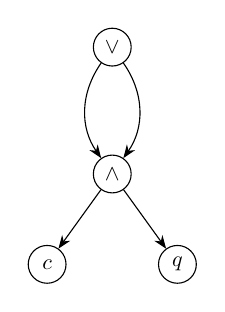
\begin{tikzpicture}[scale=0.8, transform shape, every node/.style={circle, draw, minimum size=6mm, inner sep=1pt}, >=Stealth]
            \node (or) {$\lor$};
            \node (and) [below=1.4cm of or] {$\land$};
            \node (c) [below left=1.0cm and 0.6cm of and] {$c$};
            \node (q) [below right=1.0cm and 0.6cm of and] {$q$};
            
            \draw[->] (or) to[bend right=35] (and);
            \draw[->] (or) to[bend left=35] (and);
            \draw[->] (and) -- (c);
            \draw[->] (and) -- (q);
        \end{tikzpicture}
    \end{minipage}
    \hfill
    % --- 3. Auxiliary Definitions ---
    \begin{minipage}{0.33\textwidth}
        \centering
        \textbf{3. Formula View} \\[0.5em]
        \small With auxiliary variables \\[0.5em]
        \fbox{\begin{minipage}{0.9\textwidth}
            \footnotesize
            \textbf{Auxiliary Defs:} \\[0.2em]
            $T_1 = c \land q$ \\
            $T_2 = T_1 \lor T_1$ \\[0.4em]
            \textbf{Top-Level Formula:} \\[0.2em]
            $F = T_2$
        \end{minipage}}
    \end{minipage}
    \label{fig:tree_to_dag}
\end{figure}

\textbf{Example:} simple (ripple-carry) \textit{n}-bit adder:
\begin{itemize}
	\item input numbers: $s_1, ..., s_n$ and $a_1,...,a_n$
	\item output: $s_1', ..., s_n'$
\end{itemize}

The formula with auxiliary variables $c_1, ..., c_{n+1}$: 
\[
	c_1 = 0 \land \bigwedge^{n}_{i = 1} (s'_i = s_i \oplus a_i \oplus c_i) \land (c_{i + 1} = (s_1 \land a_i) \lor (s_i \land c_i) \lor (a_i \land c_i)) 
.\] 

We can implement such definitions in hardware: route an output of one gate to multiple other gates. \\ 
To get back a tree: substitute all auxiliary variables $c_i$, but we get much bigger formula. Or, existentially quantify all auxiliary variables. 


\subsection*{Formula Representation of Sequential Circuits}

We represent sequential circuit as $C = (\bar{s}, \text{Init}, R, \bar{x}, \bar{a})$ where: 
\begin{itemize}
	\item $\bar{s} = (s_1, ..., s_n)$ is the vector of state variables
	\item \textit{Init} is a boolean formula with \textit{FV(Init)} $\subseteq \{s_1, ..., s_n\}$i
	\item $\bar{a} = (a_1, ..., a_m)$ is the vector of input variables
	\item $\bar{x} = (x_1, ..., x_k)$ is the vector of auxiliary variables (for \textit{R})
	\item \textit{R} is a boolean formula called transition formula, for which $$\text{FV(R)} \subseteq \{s_1, ..., s_n, a_1, ..., a_m, x_1, ..., x_k, s'_1, ..., s'_n\}$$
\end{itemize}
Transition system for \textit{C} is \textit{(S, I, r, A)} where $S = \{0, 1\}^{n}, A = \{0, 1\}^{m}$, 
\begin{itemize}
	\item $I = \{\bar{v} \in \{0, 1\}^{n} \, | \, [\bar{s} \mapsto \bar{v}] \models Init\}$
	\item $r = \{(\bar{v}, \bar{u}, \bar{v}') \in \{0, 1\}^{n + m +n} \, | \, [(\bar{s}, \bar{a}, \bar{s}') \mapsto (\bar{v}, \bar{u}, \bar{v})] \models \exists \bar{x} . R\}$
\end{itemize}

Auxiliary variables $\bar{x}$ are treated as existentially quantified, can use conjucts $x_i =$ \textit{E}$(\bar{s}, \bar{a}, \bar{x})$ to express intermediate values. 

\emph{\underline{What needs to be remembered}}: We can represent faithfully and, in many cases, efficiently, transition systems using propositional formulas for initial state and transition relation. 

\subsection*{Checking Inductive Invariant using SAT queries}

Given the sequential circuit representation $C = (\bar{s}, Init, R, \bar{x}, \bar{a})$ and a formula \textit{Inv} with $FV(Inv) \subseteq \{s_1, ..., s_n\}$, how do we check that \textit{Inv} is an inductive invariant? \\
Let us write \textit{negations} of conditions "$Init \subseteq Inv$" and "$r[Inv] \subseteq Inv$"
\begin{itemize}
	\item An initial state is not included in invariant: $$ Init \land \neg Inv$$
	\item There is a state satisfying invariant, leading to a state that breaks invariant: $$\underbrace{Inv}_{\bar{s}} \land \underbrace{R}_{\bar{s}, \bar{a}, \bar{x}, \bar{s}'} \land \underbrace{\neg Inv[\bar{s} := \bar{s}']}_{\bar{s}'$$
	Note that $\bar{a}, \bar{x}$ variables are also existentially quantified, as they should be. 
\end{itemize}

We can check if a formula is an inductive invariant using two queries to a SAT solver and making sure that they both return \textbf{unsat}. 

\newpage
\begin{center}
  {\LARGE \textbf{Appendix: Scala Snack Dispenser}}
\end{center}
\vspace{0.5cm}

\subsection*{Description}
Snack dispenser has 6 levels with 4 slots each. Each slot can hold 10 items. Each item costs 2 CHF. The only way to operate a machine is to insert 1 CHF coin into temporary storage (one step), which must be done two times, then select the refreshment (in one step), which immediately dispenses the snack or cancels and returns coins if none is available in the slot, or if the stable coin storage is full. The machine can hold up to 500 CHF in its stable coin storage. It starts full with items but with no coins. Describe this transition system and estimate the cardinality of the set of all of its states. Can the stable storage ever hold 99 coins? 100 coins? 490 coins?

states: $10^{4 \cdot 6} \cdot 501 \cdot 2 = 10^{24} \cdot 1002 > 10^{27}$ 

coins: $0 \rightarrow 2 \rightarrow ... \rightarrow 98 \rightarrow 100 \rightarrow 240 \cdot 2 = 480
\subsection*{Code}
\begin{lstlisting}[language=Octave]
import stainless.lang._
import stainless.collection._
object Dispenser {
  abstract sealed class Action
  case class FirstCoin() extends Action
  case class SecondCoin(levelNo: BigInt, slotNo: BigInt) extends Action {
    require(0 <= levelNo && levelNo <= 5 &&
            0 <= slotNo && slotNo <= 3)
  }

  case class State(
    levels: List[List[BigInt]],
    coins: BigInt,
    oneInserted: Boolean)
  {
    require(levels.size == 6 &&
            levels.forall(l => l.size == 4) &&
            0 <= coins && coins <= 500)
  }

  def isInitial(s: State): Boolean = {
    s.levels.forall(l => l.forall(itemNo => itemNo==10)) &&
    s.coins == 0 &&
    s.oneInserted == false
  }

  def r(s1: State, a: Action): Option[State] = {
    a match {
      case FirstCoin() if !s1.oneInserted && s1.coins < 500 =>
        Some(s1.copy(
          oneInserted = true,
          coins = s1.coins + 1))
      case SecondCoin(levelNo,slotNo) if s1.oneInserted && s1.coins < 500 => {
        val level: List[BigInt] = s1.levels(levelNo)
        val amount = level(slotNo)
        if (amount > 0) {
          val newLevel: List[BigInt] = level.updated(slotNo, amount - 1)
          Some(s1.copy(
            levels = s1.levels.updated(levelNo, newLevel),
            oneInserted = false,
            coins = s1.coins + 1))
        } else None()
      }
      case _ => None()
    }
  }

  def isTraceLike(t: List[(State,Action)]): Boolean = {
    t match {
      case Cons((s1,a1), Cons((s2,a2),rest)) => {
        if (r(s1,a1)==Some(s2)) isTraceLike((s2,a2)::rest)
        else false
      }
      case _ => true
    }
  }

  def isTrace(t: List[(State, Action)]): Boolean = { // last action is ignored
    t match {
      case Cons((s,a),_) => isInitial(s) && isTraceLike(t)
      case _ => false
    }
  }

  def exampleTrace: List[(State,Action)] = {
    val b10 = BigInt(10)
    val s0 = State(
      levels = List(
        List(b10,b10,b10,b10),
        List(b10,b10,b10,b10),
        List(b10,b10,b10,b10),
        List(b10,b10,b10,b10),
        List(b10,b10,b10,b10),
        List(b10,b10,b10,b10)),
      coins = BigInt(0),
      oneInserted=false)
    val Some(s1) = r(s0, FirstCoin())
    val Some(s2) = r(s1, SecondCoin(0,0))
    List[(State,Action)]((s0, FirstCoin()), (s1, SecondCoin(0,0)), (s2, FirstCoin()))
  }.ensuring(res => isTrace(res))

  def prop(s: State): Boolean = {
    s.coins % 2 == (if (s.oneInserted) BigInt(1) else BigInt(0))
  }

  def propInductive(t: List[(State, Action)]): Unit = {
    require(isTraceLike(t) &&
      (t match {
        case Cons((s,a),_) => prop(s)
        case _ => false
      })
    )
    t match {
      case Cons((s,a),Nil()) => ()
      case Cons((s,a),rest) => {
        assert(rest.last == t.last)
        propInductive(rest)
      }
    }
  }.ensuring(_ => prop(t.last._1))

  def propInvariant(t: List[(State, Action)]): Unit = {
    require(isTrace(t))
    propInductive(t)
  }.ensuring(_ => prop(t.last._1))
}
\end{lstlisting}
\end{document}
